\chapter{Produktudvikling}\label{Produktudvikling} 

\section{Systemarkitektur}\label{Systemarkitektur}
Der er udarbejdet forskellige arkitektur-diagrammer på baggrund af de specificerede systemkrav. Diagrammerne har til formål at beskrive Automatisk Ultralydsscanner som et overordnet system.

Arkitekturen beskriver den grundlæggende organisering af Automatisk Ultralydsscanner og opbygningen af dens tilhørende PC Applikation. Der er i diagrammerne designet ud fra, at 3D kamera er af typen Microsoft Kinect 2.0 og Robotarm er en Universal Robot UR10 robot. For detaljeret gennemgang af systemarkitektur for Automatisk Ultralydsscanner se Bilag  \ref{Udviklingsdokument} Dokumentation.

\subsection{Domænemodel}
Nedenstående domænemodel på figur \ref{domain} viser de overordnede moduler og tydeliggør forbindelserne samt interaktionerne mellem de forskellige aktører i Automatisk Ultralydsscanner. 

\begin{figure}[H]
    \centering
    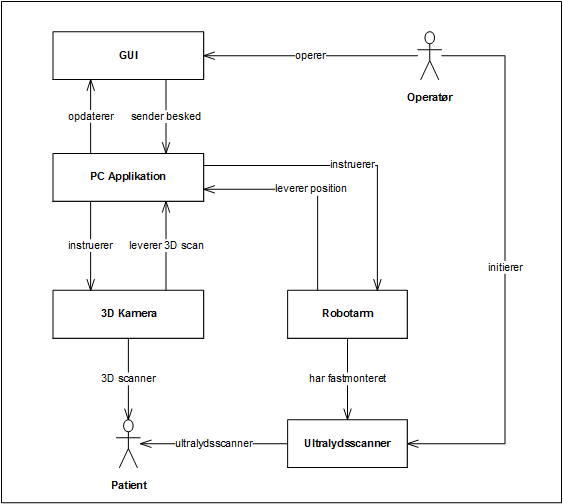
\includegraphics[width=0.6\textwidth]{figurer/d/Design/uml_domain}
    \caption{Domænemodel for Automatisk Ultralydsscanner}
    \label{domain}
\end{figure}

\subsection{Block Definition Diagram}
Automatisk Ultralydsscanner består af Robotarm, en computer, et Access Point, 3D kamera og Ultralydsscanner. Access Point er medtaget for at sikre at Robotarm har samme IP-adresse. Det er vigtigt at bemærke, at computer skal have PC Applikation installeret og en mus og en skærm for at Operatør kan integrere med PC Applikation. Block Definition Diagrammet på figur \ref{BDD}, viser hvordan systemets blokke er forbundet. 

\begin{figure}[H]
    \centering
    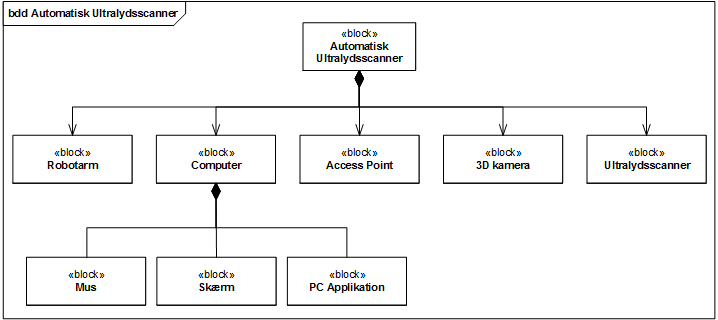
\includegraphics[width=1\textwidth]{figurer/d/Design/BDD}
    \caption{BDD for Automatisk Ultralydsscanner}
    \label{BDD}
\end{figure}

\subsection{Internal Block Diagram}
Detaljerne i interaktionen mellem de enkelte blokke er beskrevet i Internal Block Diagram i figur \ref{IBD}, som viser systemets interne forbindelser og flow mellem de forskellige blokke. Bemærk at Ultralydsscanner ikke er inkluderet her, da den ikke har forbindelse til de andre blokke udover at være monteret mekanisk på Robotarm. Forbindelsen mellem PC Applikation og Access Point, samt Acces Point og Robotarm er oprettet med ethernet-kabler. 3D kamera forbindes til PC Applikation gennem USB. For simplificering er PC, Mus og Skærm fra BDD undladt.

\begin{figure}[H]
    \centering
    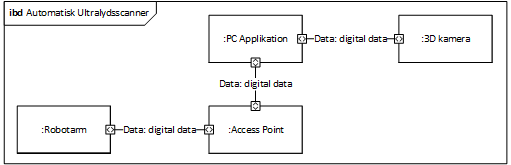
\includegraphics[width=0.8\textwidth]{figurer/d/Design/IBD}
    \caption{IBD for Automatisk Ultralydsscanner}
    \label{IBD}
\end{figure}

\subsection{Pakkediagram}
For at se et overblik over afhængighederne mellem store moduler (pakker) i PC Applikation, se figur \ref{pakke} nedenfor. Der blev identificeret behovet for en GUI (AutoSonographyWPF), indhentning af en 3D scanning fra 3D kamera (ComputerVisionLibrary), beregning af positioner og rotationer på baggrund af en 3D scanning (CalculationLibrary), samt at sende positurer til Robotarm (RoboLibrary). \newline
De forskellige biblioteker anvender fælles datastrukturer som blev samlet i ét bibliotek for at undgå cykliske forbindelser (DataStructures). Bemærk at AutoSonographyWPF afhænger af alle bibliotekerne, men at de tre hovedbiblioteker ikke afhænger af hinanden.

\begin{figure}[H]
    \centering
    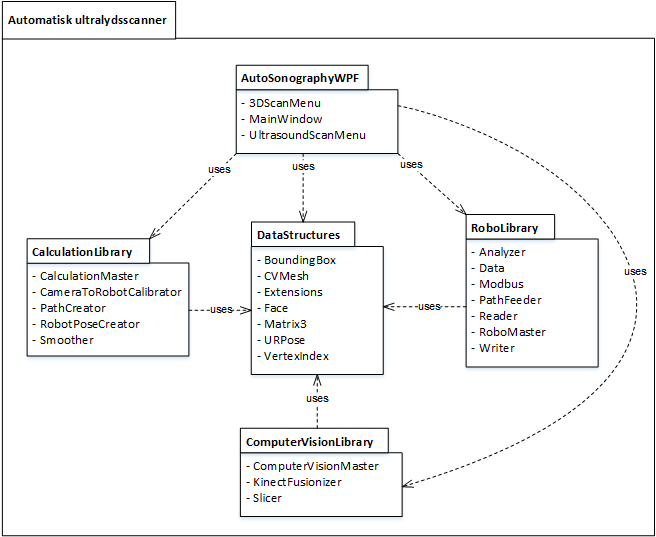
\includegraphics[width=1\textwidth]{figurer/d/Design/Pakkediagram}
    \caption{Pakkediagram for PC Applikation}
    \label{pakke}
\end{figure}

\newpage
\section{Systemdesign} \label{Systemdesign}
Systemdesignet beskriver hvordan PC Applikations individuelle moduler er opbygget og hvordan disse interagerer med hinanden.  
Nedenfor vil relevante diagrammer blive gennemgået. For detaljeret gennemgang af systemdesign for Automatisk Ultralydsscanner se Bilag \ref{Udviklingsdokument} Udviklingsdokument.

Klassediagrammerne viser strukturen i PC Applikations klasser og afhængighederne mellem disse. Hver klasse i diagrammerne indeholder de vigtigste metoder og attributer fra klassen, der udgør funktionaliteten i PC Applikation. Opbygningen er valgt for at skabe høj samhørighed og lav kobling - men også med den tanke at hele eller dele af projektet skal kunne genbruges.

For et overblik over funktionaliteten i PC Applikation kan der tages udgangspunkt i klassediagrammet for den grafiske brugergrænseflade på figur \ref{class_gui}. Beskrivelser følger på næste side. 

\begin{figure}[H]
    \centering
    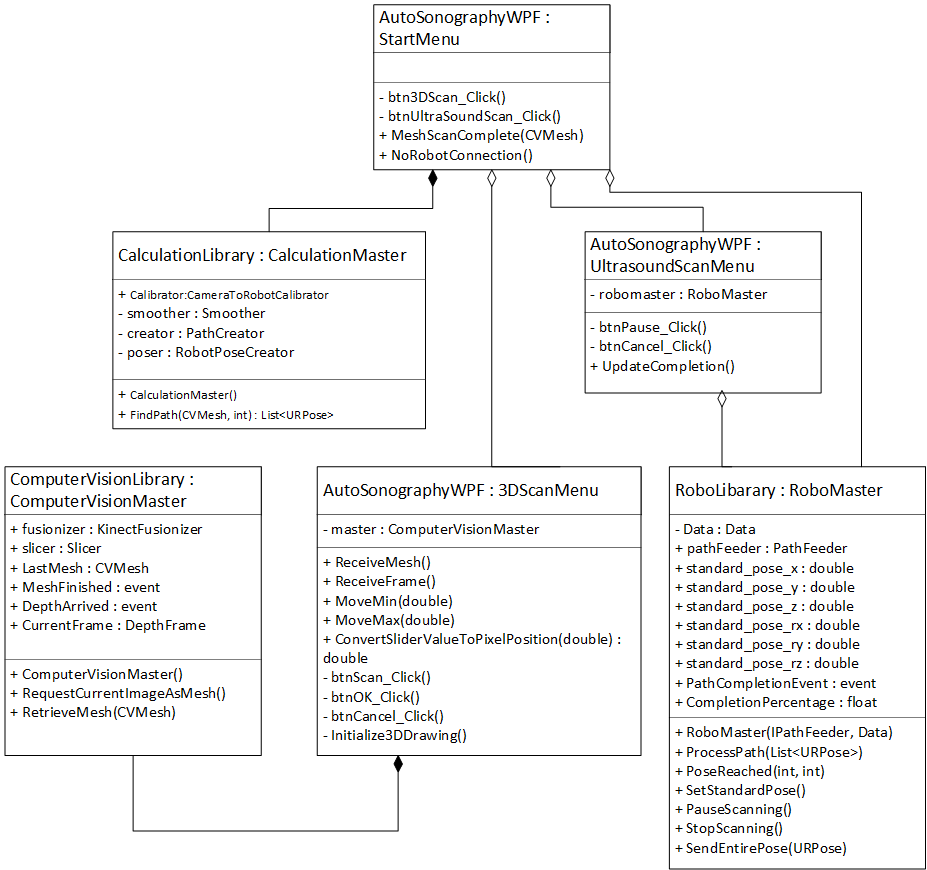
\includegraphics[width=1\textwidth]{figurer/d/Design/Class/uml_class_gui}
    \caption{Klassediagram for GUI}
    \label{class_gui}
\end{figure}
\newpage

\let\labelitemi\labelitemii
\begin{itemize}
\item{MainWindow}\newline
Giver anledning til at foretage et 3D scan. Såfremt en 3D scanning er gennemført giver det også anledning til at starte en ultralydsscanning. Når denne menu startes, oprettes en instans af RoboMaster, for at sætte Robotarm i standard positur. Dette er nødvendigt, hvis Robotarm ikke står i standard positur, da den ville kunne hindre en 3D scanning, fordi den eventuelt blokerer for 3D kameras syn.
Hvis der ikke er nogen forbindelse til Robotarm vil der vises en besked om dette.

\item{3DScanMenu}\newline
I denne menu er der mulighed for at se det nuværende dybdebillede, afgrænse området der skal 3D scannes og foretage en 3D scanning.

\item{UltrasoundScanMenu}\newline
I denne menu kan den procentvise færdiggørelse af ultralydsscanningen følges. Der er også mulighed for at pause samt afbryde ultralydsscanningsprocessen.

\item{ComputerVisionLibrary}\newline
Dette bibliotek har til formål at indhente en 3D scanning fra 3D kamera og afgrænse scanningen ift. de parametre der er givet med fra 3DScanMenu.

\item{CalculationLibrary}\newline
I dette bibliotek anvendes en 3D scanning fra ComputerVisionLibrary. CalculationMaster har til formål at finde de positurer til Robotarm, der er nødvendige for at kunne fuldføre en ultralydsscanning.

\item{RoboLibrary}\newline
Biblioteket giver mulighed for at kommunikere med Robotarm. Her sættes dens acceleration, hastighed og positur.
\end{itemize}

Her skal det nævnes at de lavestliggende kommunikationsklasser i RoboLibrary er lånt fra et tidligere bachelorprojekt (TRU). Klasserne er kopieret og skrevet til, så de passer ind i PC Applikation. Såfremt andet kode er kopieret, er det nævnt i koden med en reference til kilden.
For at få en dybere forståelse af logik og data-kommunikationen i ComputerVisionLibrary, CalculationLibrary samt RoboLibrary, se klassediagrammerne for de enkelte biblioteker i bilag \ref{Klassediagram} Udviklingsdokument. 
\newpage

\subsection{3D behandling}
En vigtig del af produktet er bindeledet mellem 3D kamera og Robotarm. Efter scanningen er foretaget, er det næste skridt at finde ud af hvor Robotarm skal bevæge sig hen. På figur \ref{seq_pathcreation} ses processen for de trin der skal til for at gøre dette. CalculationMaster virker som en grænseflade mellem GUI'en (MainWindow) og de underliggende 3D-behandlingsklasser. CameraToRobotCalibrator sørger for at placere 3D scanningen i Robotarms rum. Da der kan forekomme ujævnheder i scanningen, vil Smoother forsøge at jævne disse ud. PathCreator finder interessante punkter i scanningen, der skal til for at afdække brystet i en ultralydsscanning, j.f. figur \ref{Probensbevagelse} på side \pageref{Probensbevagelse}. Til sidst ekstrapoleres punkterne, så det passer med at Robotarm vil være roteret mod punkterne i 3D scanningen med et offset der svarer til ultralydsprobens længde.
Disse positurer gives tilbage til MainWindow, for senere at blive sendt videre til Robotarm. 
Denne opdeling af processen er valgt så enkelte moduler kan udskiftes eller forbedres uden at skulle ændre meget i koden.
\begin{figure}[H]
    \centering
    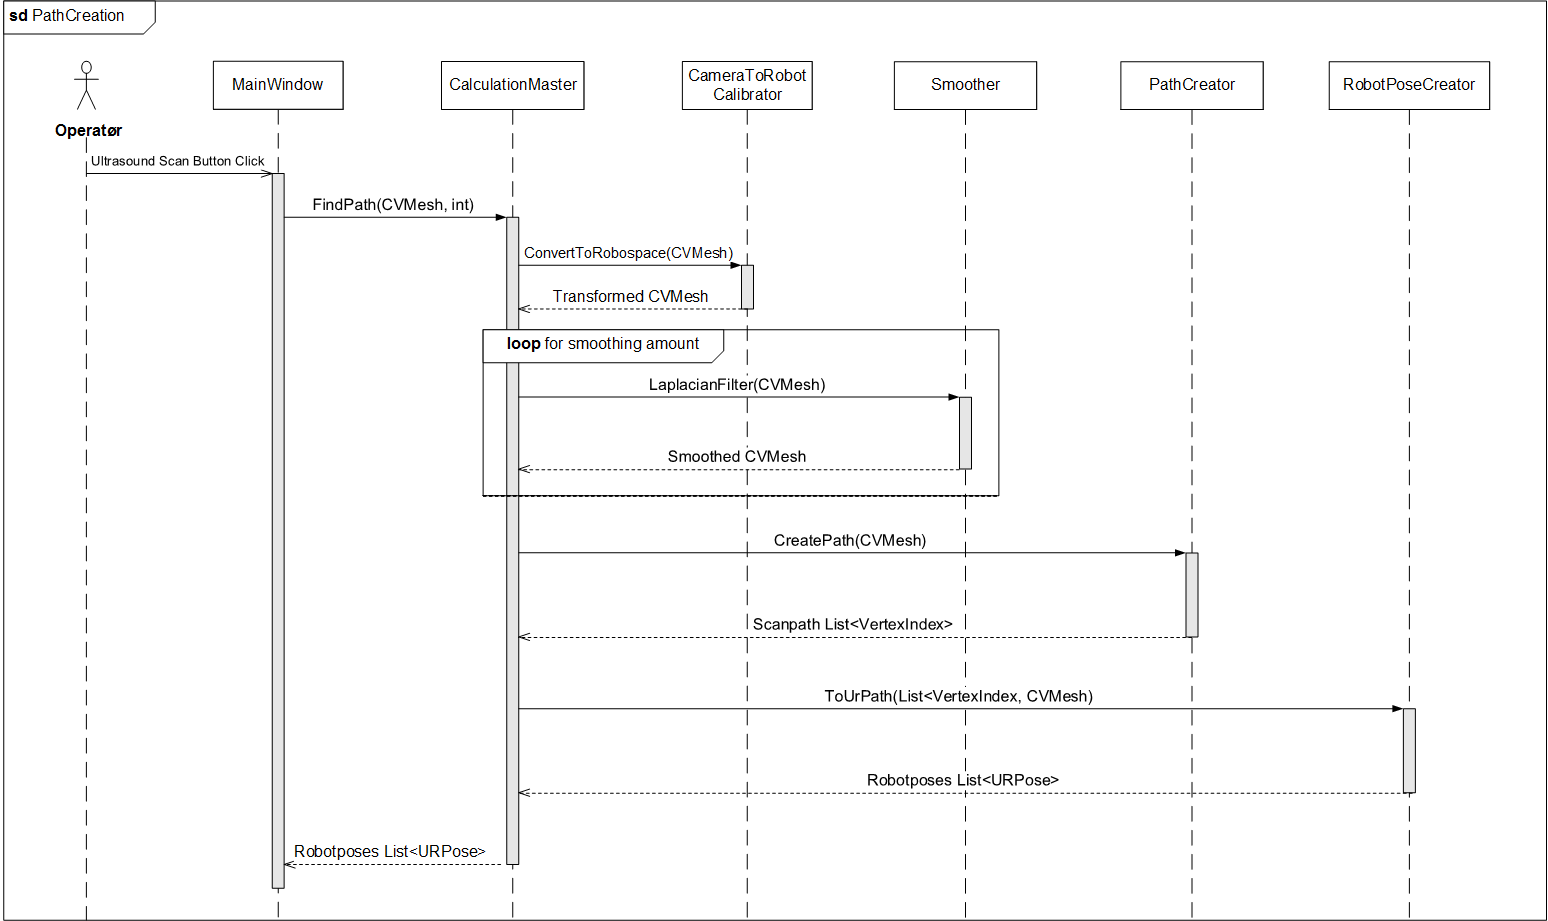
\includegraphics[width=1\textwidth]{figurer/d/Design/Sequence/sd_pathcreation}
    \caption{Sekvensdiagram for 3D Path Creation}
    \label{seq_pathcreation}
\end{figure}
\newpage
\section{Implementering}
I dette afsnit omtales de det implementerede hardware samt software der er nødvendige for at realisere Automatisk Ultralydsscanner.
Prototype-versionen af produktet inkluderer: Robotarm af typen Universal Robots 10, 3D kamera af typen Microsoft Kinect 2.0, Access Point af typen D-Link DAP-1160, og PC Applikation som en WPF applikation programmeret i C\#.
\subsection{Hardware}
Opstillingen af Automatisk Ultralydsscanner ses på figur \label{setup} og som en skitse på figur \label{3dsetup}, hvor forbindelserne til den PC der har PC Applikation er udeladt. 

\begin{figure}[H]
  \centering
  \begin{minipage}{0.4\textwidth}
    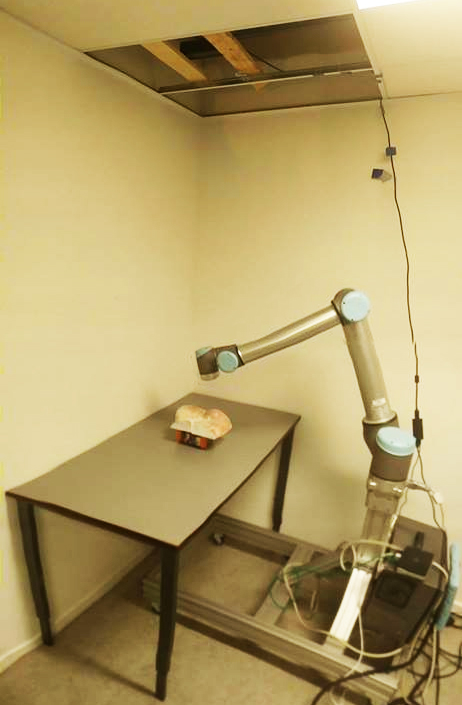
\includegraphics[width=\textwidth]{figurer/setup}
    \caption{Opstilling}
    \label{setup}
  \end{minipage}
  \hfill
  \begin{minipage}{0.4\textwidth}
    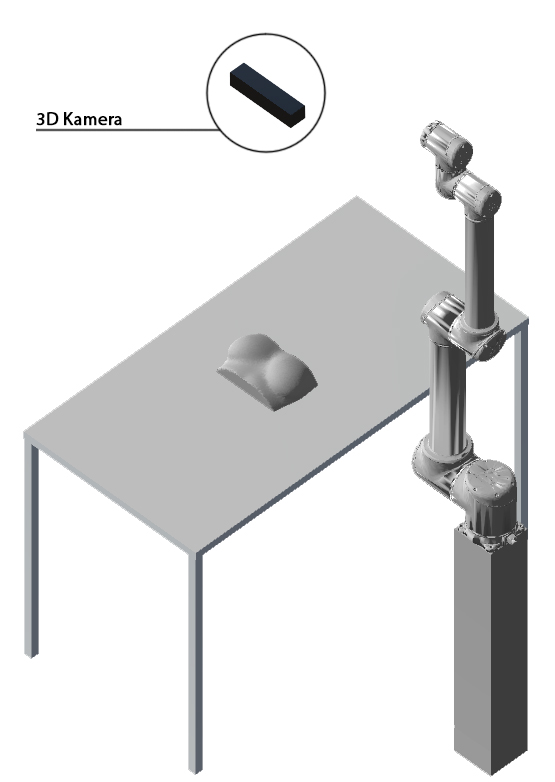
\includegraphics[width=\textwidth]{figurer/3d_setup}
    \caption{Opstillingsskitse}
    \label{3dsetup}
  \end{minipage}
\end{figure}

Der blev ikke udviklet noget nyt hardware til Automatisk Ultralydsscanner - altså blev der kun brugt det ovennævnte eksisterende hardware. Valget for UR10 blev dannet på baggrund af dens arms spændvidde, da fx UR5 ville være for lille til dette projekt. Grundlaget for Microsoft Kinect som 3D kamera uddybes i næste sektion.
\newpage
\subsection{Software}
PC Applikation er opbygget som en Visual Studio solution, hvor hver pakke fra pakkediagrammet, vist på figur \ref{pakke} på side \pageref{pakke}, er implementeret som projekter. Projektet der startes i solutionen, og dermed er det eksekverbare program der skal køres, er WPF-projektet 'AutoSonographyWPF'. \newline
Der blev brugt meget tid på at finde et computervision-bibliotek der kunne bruges til 3D scannings-forløbet, givet et vilkårligt 3D kamera. Da det blev konstateret at Microsoft's eget API fungerede sammen med Microsoft Kinect 2.0, og at denne havde adskillige funktioner der var vitale for Automatisk Ultralydsscanner, faldte valget på dette som API, og Microsoft Kinect 2.0 som 3D kamera. 
Valget for at programmere PC Applikation i C\# er dannet på baggrund af at: 
\begin{itemize}
\item Lånt kode til kommunikation med Robotarm i RoboLibrary er programmeret i .NET/C\#
\item Kinect API'et understøtter C\#
\item Der er tidligere kendskab til WPF, .NET og C\# generelt
\end{itemize}

Kinect API'et er inkluderet i solutionen som .dll-filer.

Solutionen indeholder også en række testprojekter med unittests som beskrives nærmere i bilag \ref{Udviklingsdokument} Dokumentation, i afsnit 'Test'. For at se hvilke udviklingsværktøjer der blev brugt, se bilag \ref{Udviklingsdokument} Dokumentation, i afsnit 'Udviklingsmiljø'. Kildekoden er vedlagt som bilag \ref{Kildekode}.